\newpage
% ============================================================
%  ANEXOS: Experimentos complementarios
% ============================================================
\section*{Anexos}
\addcontentsline{toc}{section}{Anexos}

Los siguientes experimentos se realizaron como extensi\'{o}n del an\'{a}lisis
principal, explorando datasets adicionales para verificar la robustez de
los estimadores VT y LD, y del clasificador mono/multifractal en dominios
no cubiertos por las actividades principales del trabajo.

% ------------------------------------------------------------
\subsection*{A.1 Deuda soberana: rendimiento del Tesoro a 10 a\~{n}os (FRED DGS10)}
% ------------------------------------------------------------

\textbf{Motivaci\'{o}n.} Las tasas de inter\'{e}s soberanas constituyen un
sistema financiero de naturaleza institucional, donde la pol\'{i}tica
monetaria genera memoria persistente mediante suavizaci\'{o}n deliberada de
tasas. A diferencia de la volatilidad burs\'{a}til (Actividad~6), que refleja
expectativas agregadas de millones de agentes, las tasas soberanas
capturan la ``memoria institucional'' de la autoridad monetaria.

\textbf{Dataset.} Serie diaria \texttt{DGS10} del repositorio FRED
(Federal Reserve Economic Data), $n = 16\,801$ observaciones desde el
2 de enero de 1962 hasta el 26 de mayo de 2026. Los niveles en porcentaje
($\mu = 5{,}8139\,\%$, $\sigma = 2{,}9353\,\%$) exhiben
autocorrelaci\'{o}n de primer orden $\text{ACF}(1) = 0{,}9998$, indicio de
ra\'{i}z unitaria. El an\'{a}lisis fractal se aplic\'{o} a las diferencias diarias
$\Delta \text{DGS10}_t$ para garantizar estacionariedad.

\textbf{Resultados.}
\begin{itemize}[leftmargin=2em, nosep]
    \item VT: $\hat{H} = 0{,}5185$ $[0{,}5084;\; 0{,}5286]$,
          $R^2_{\text{VT}} = 0{,}9858$.
    \item LD: $\hat{H} = 0{,}5826$, $\alpha = 0{,}1652$.
    \item Clasificador: $R^2_{\tau} = 0{,}8925$ \textrightarrow\ multifractal.
\end{itemize}

\textbf{Interpretaci\'{o}n.} La memoria persistente es modesta
($H \approx 0{,}52$), apenas por encima del umbral de independencia. La
pol\'{i}tica monetaria, aunque suaviza las tasas en niveles, introduce
ruido en las diferencias que diluye la LRD. El resultado multifractal
sugiere que diferentes reg\'{i}menes monetarios (crisis vs.~estabilidad)
exhiben din\'{a}micas de escalamiento distintas.

\begin{figure}[H]
    \centering
    \begin{minipage}[t]{0.48\textwidth}
        \centering
        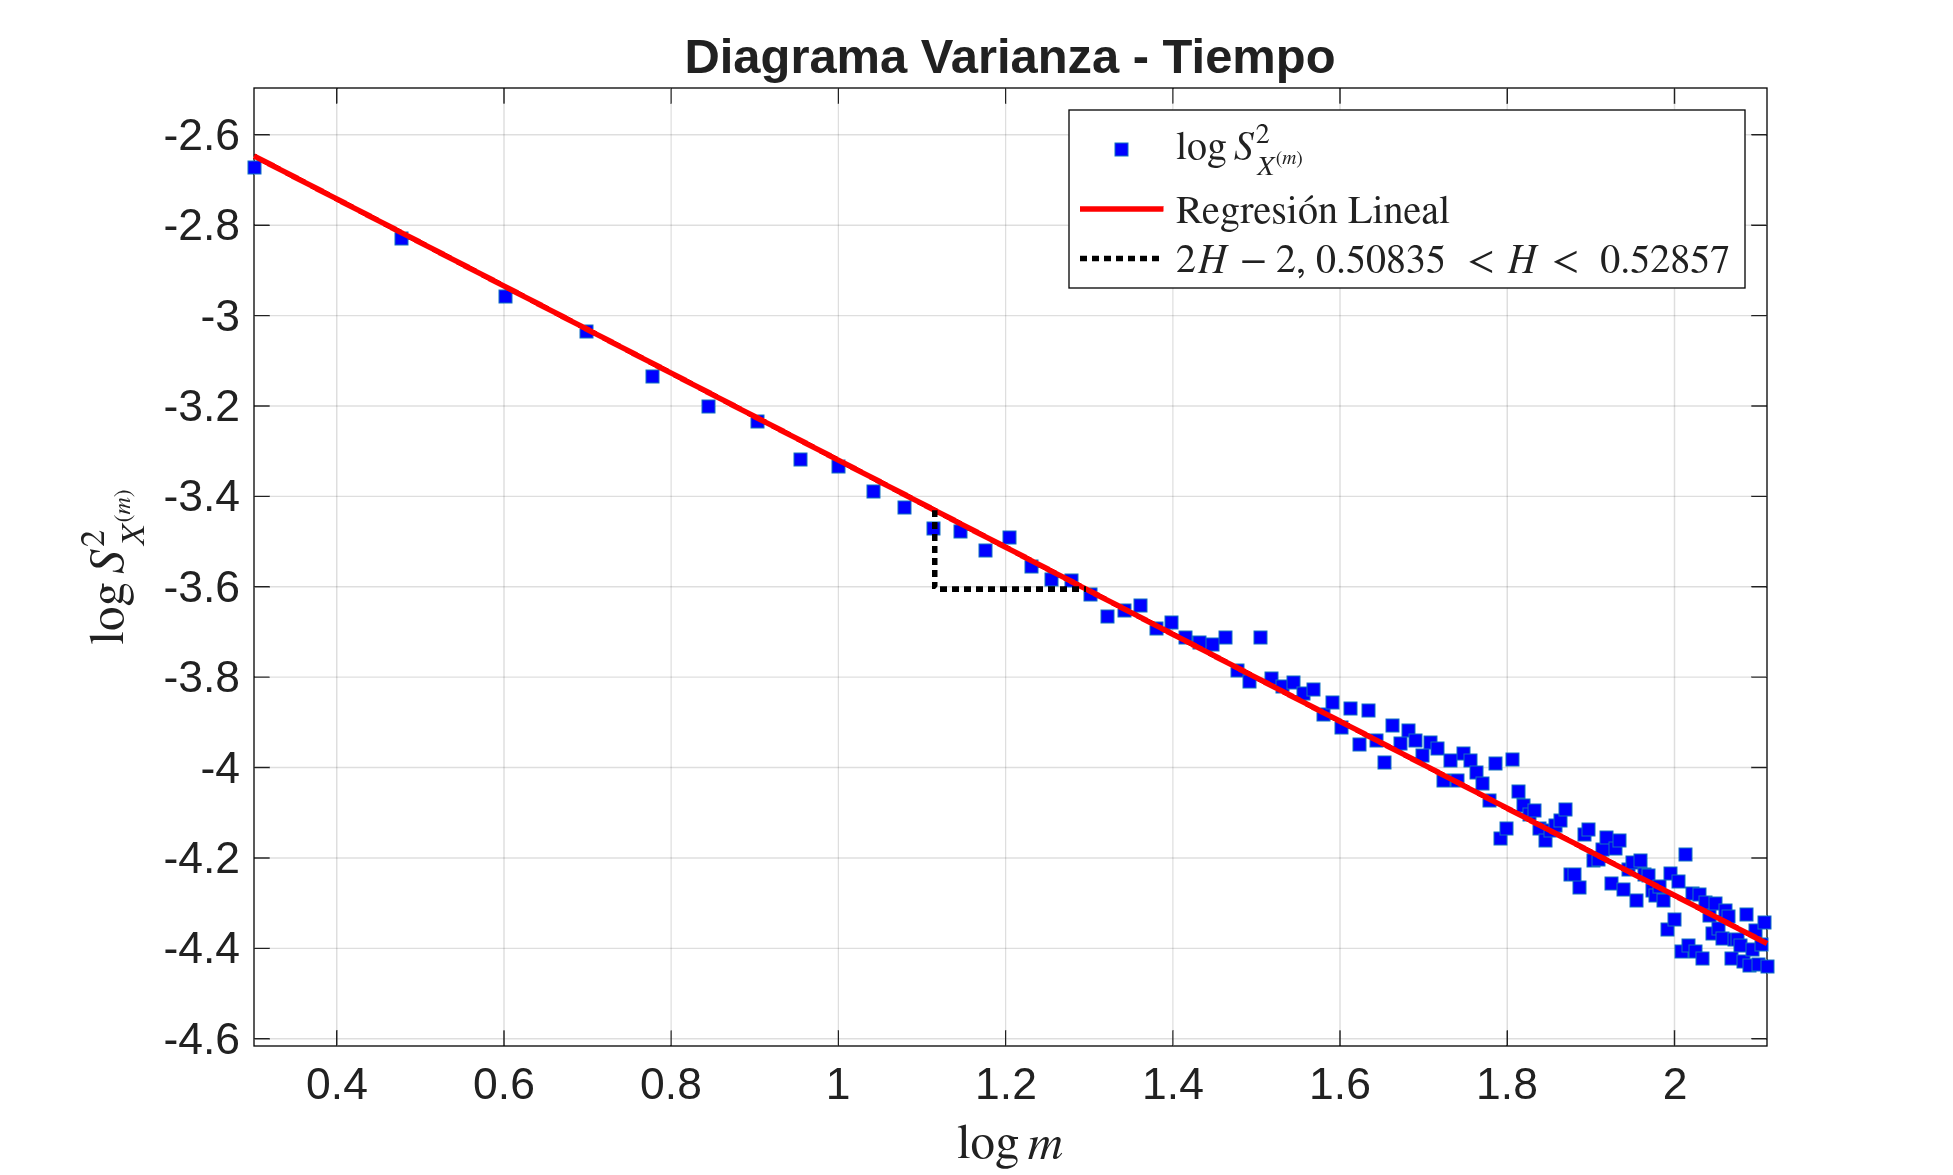
\includegraphics[width=\textwidth]{actividades/actividad6/imgs/dgs10_diagrama_vt.png}
        \caption{Anexo A.1: Diagrama VT de diferencias DGS10.}
    \end{minipage}
    \hfill
    \begin{minipage}[t]{0.48\textwidth}
        \centering
        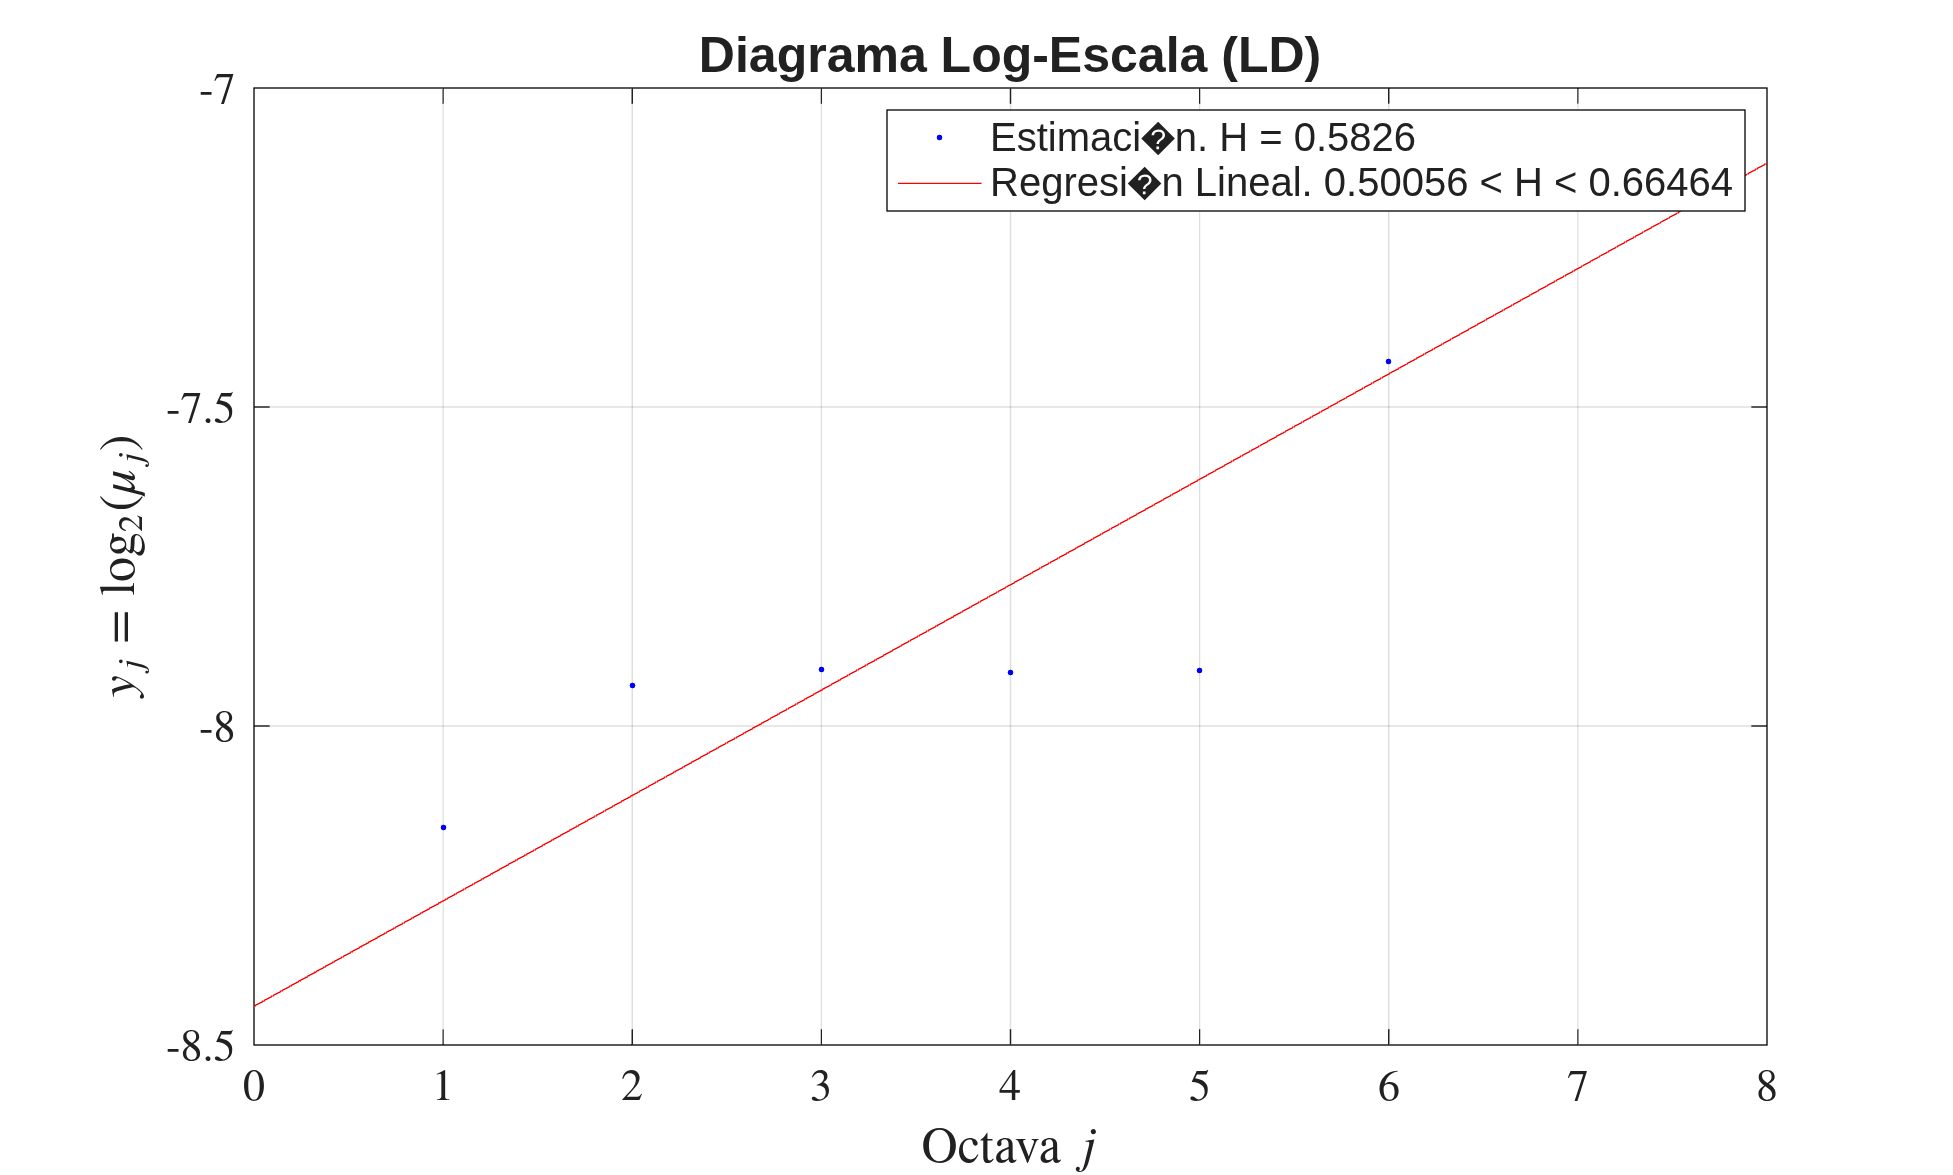
\includegraphics[width=\textwidth]{actividades/actividad6/imgs/dgs10_diagrama_ld.png}
        \caption{Anexo A.1: Diagrama LD de diferencias DGS10.}
    \end{minipage}
\end{figure}

\begin{figure}[H]
    \centering
    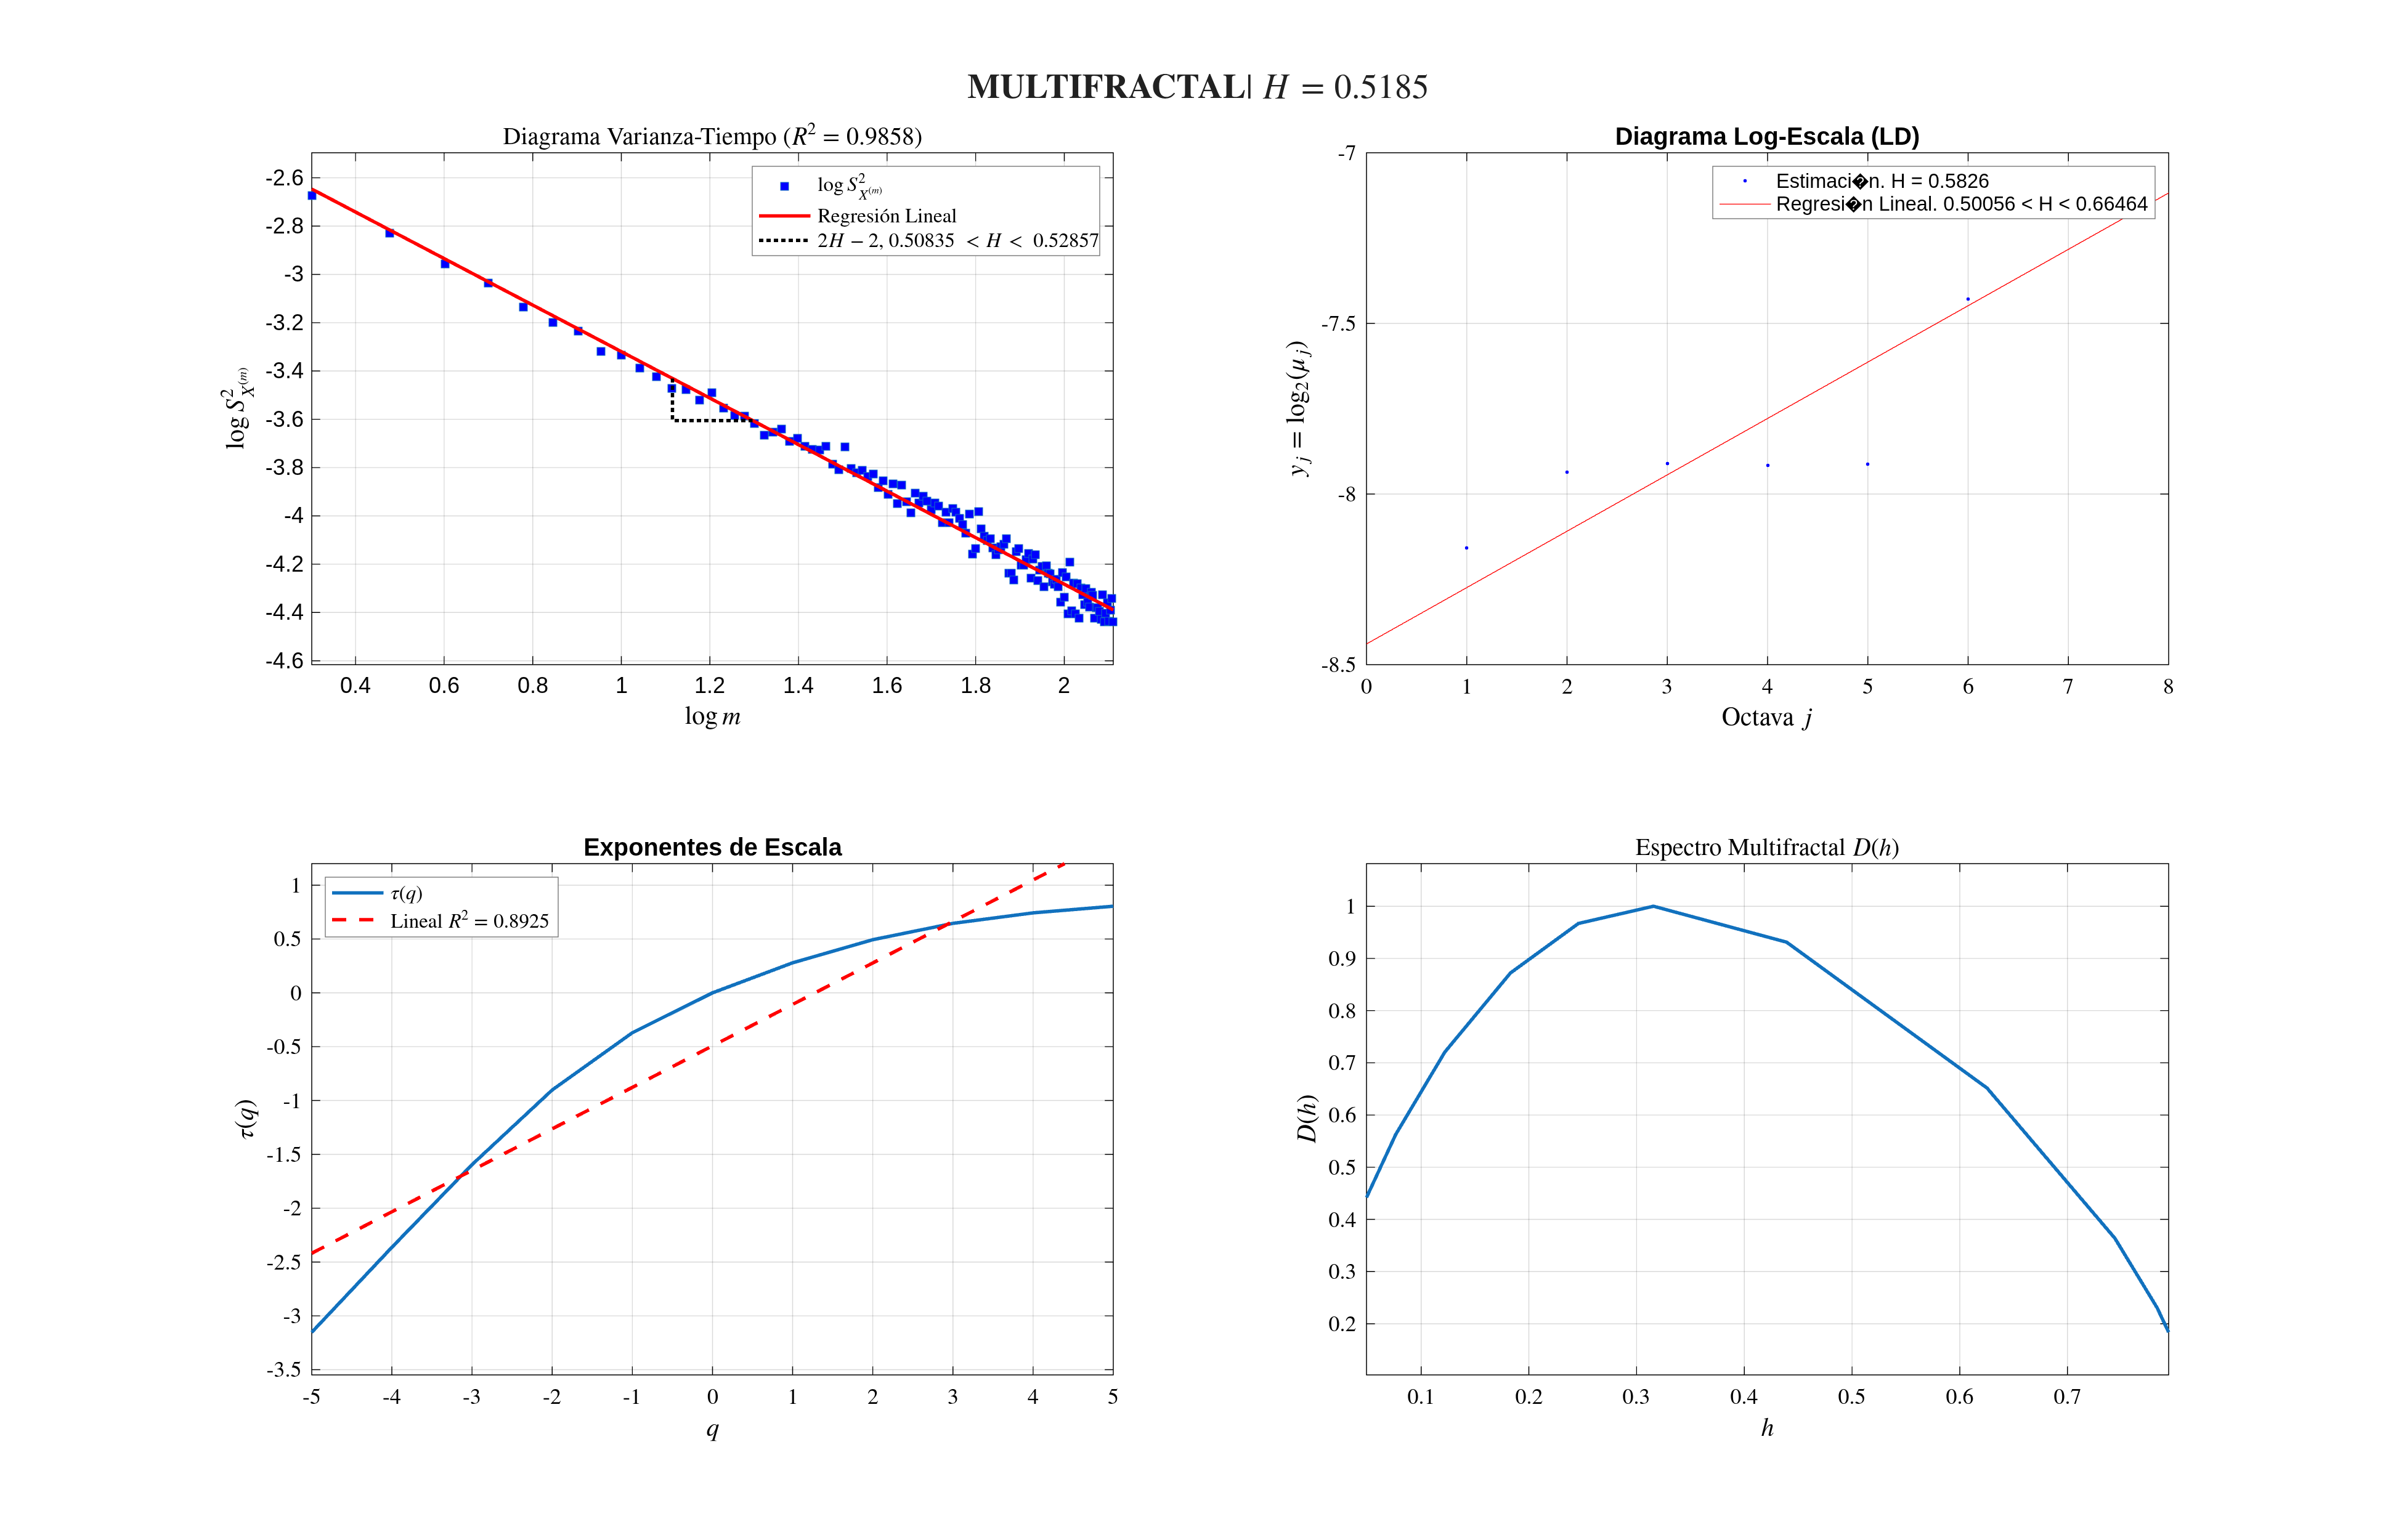
\includegraphics[width=0.85\textwidth]{actividades/actividad6/imgs/dgs10_clasificacion_fractal.png}
    \caption{Anexo A.1: Clasificaci\'{o}n multifractal de diferencias DGS10.}
\end{figure}

% ------------------------------------------------------------
\subsection*{A.2 Criptoactivos: volatilidad de Bitcoin (BTC/USDT)}
% ------------------------------------------------------------

\textbf{Motivaci\'{o}n.} Bitcoin opera como un sistema financiero
puramente digital, descentralizado y abierto 24/7, sin autoridad central
ni cierres de mercado. Desde la perspectiva del an\'{a}lisis fractal,
constituye un paradigma de sistema complejo autoorganizado donde millones
de agentes (traders, algoritmos, \textit{market makers}) interact\'{u}an sin
coordinador central.

\textbf{Dataset.} Retornos logar\'{i}tmicos de BTC/USDT en temporalidad de
1 minuto, descargados desde la API p\'{u}blica de Binance,
$n = 4\,999$ observaciones (24--28 de mayo de 2026). La volatilidad
realizada $|r_t|$ se deriv\'{o} de los retornos para capturar la LRD en la
magnitud de las fluctuaciones, siguiendo el mismo protocolo aplicado al
S\&P~500 en la Actividad~6.

\textbf{Resultados.}
\begin{itemize}[leftmargin=2em, nosep]
    \item VT: $\hat{H} = 0{,}8365$ $[0{,}8292;\; 0{,}8439]$,
          $R^2_{\text{VT}} = 0{,}9661$.
    \item LD: $\hat{H} = 0{,}6706$, $\alpha = 0{,}3411$.
    \item Clasificador: $R^2_{\tau} = 0{,}9092$ \textrightarrow\ multifractal.
\end{itemize}

\textbf{Interpretaci\'{o}n.} La volatilidad de Bitcoin exhibe memoria
persistente comparable a la del S\&P~500 ($H \approx 0{,}84$), confirmando
que la LRD en la volatilidad es una propiedad transversal de los mercados
financieros, independientemente de la naturaleza del activo (tradicional
vs.~digital). La clasificaci\'{o}n multifractal indica que episodios de alta
volatilidad (\textit{flash crashes}) y periodos de consolidaci\'{o}n operan
con din\'{a}micas de escalamiento local distintas.

\begin{figure}[H]
    \centering
    \begin{minipage}[t]{0.48\textwidth}
        \centering
        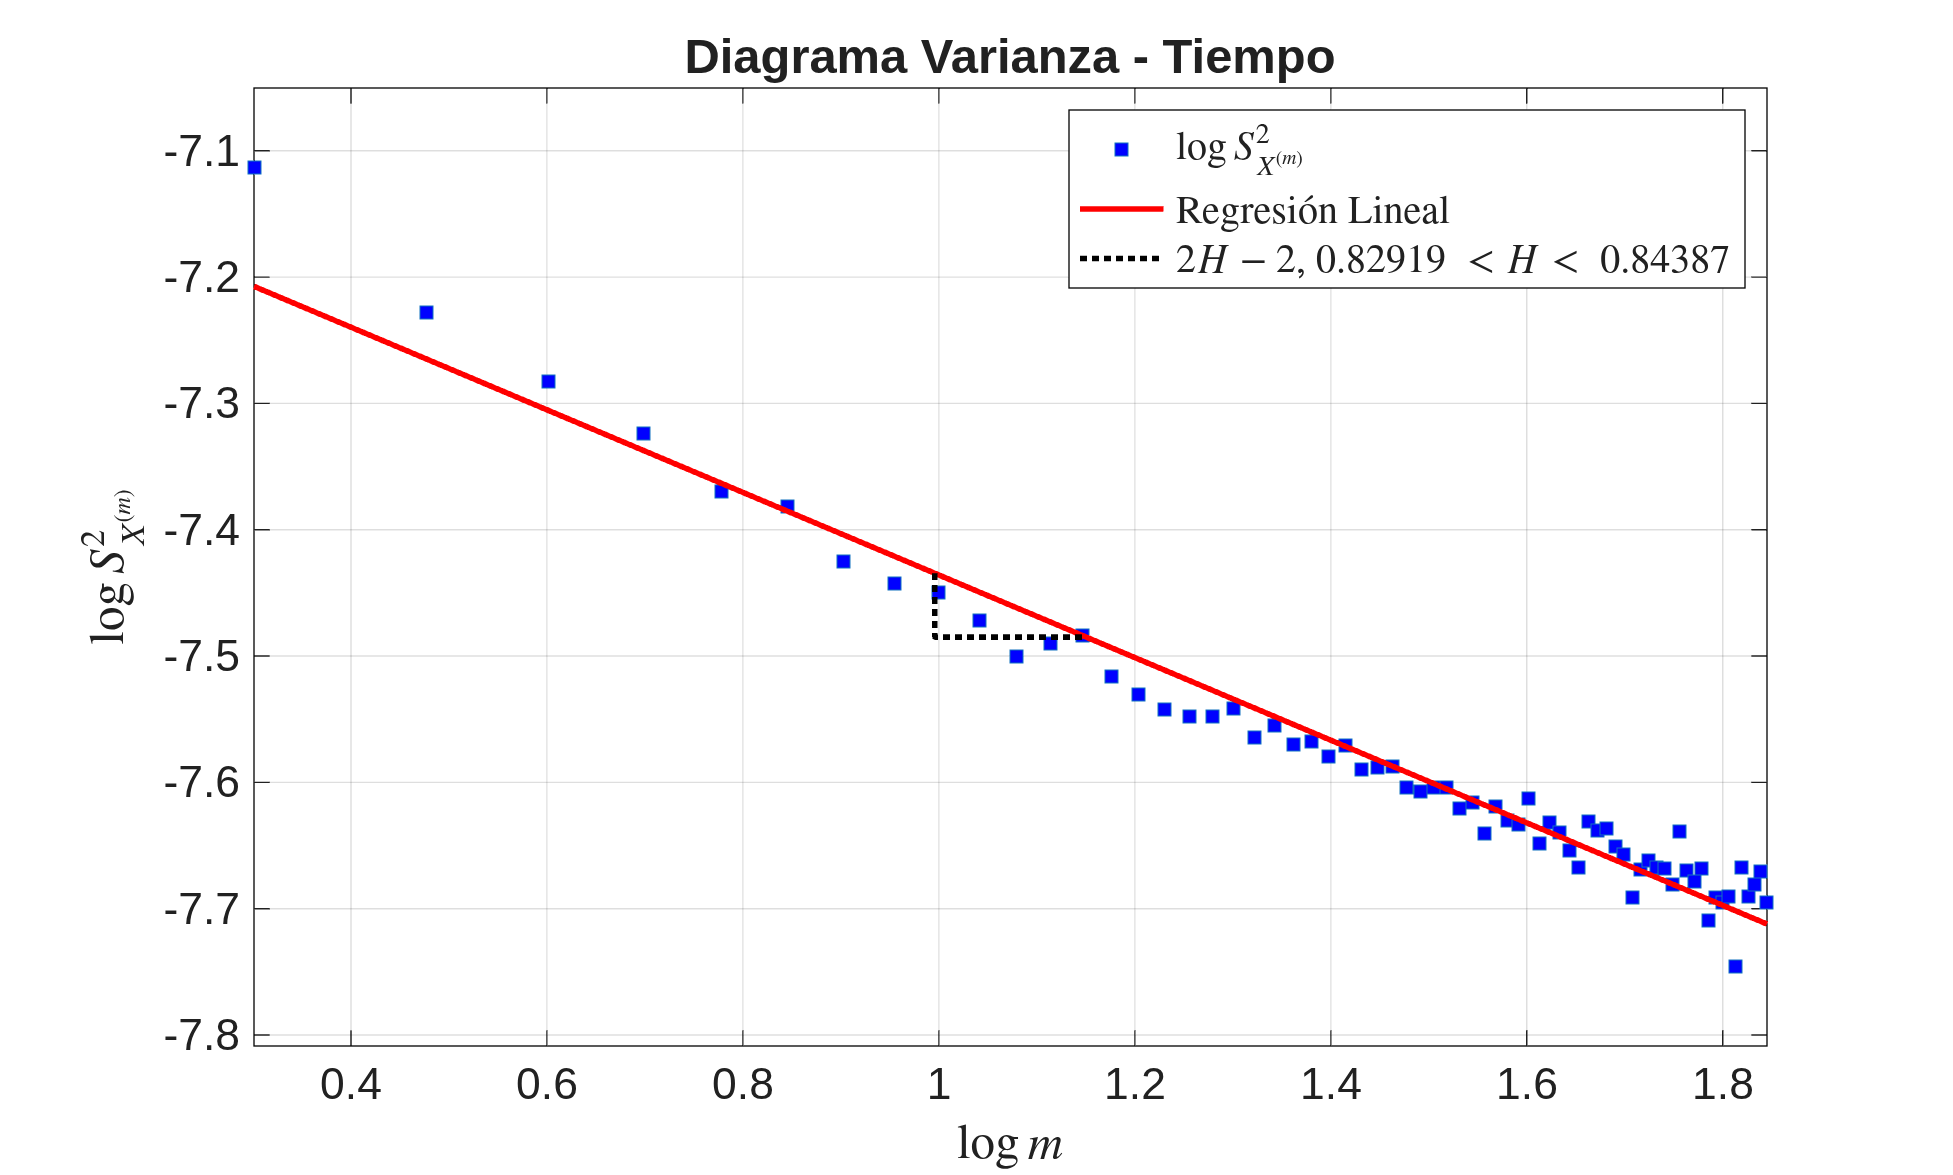
\includegraphics[width=\textwidth]{actividades/actividad6/imgs/btc_diagrama_vt.png}
        \caption{Anexo A.2: Diagrama VT de volatilidad BTC/USDT.}
    \end{minipage}
    \hfill
    \begin{minipage}[t]{0.48\textwidth}
        \centering
        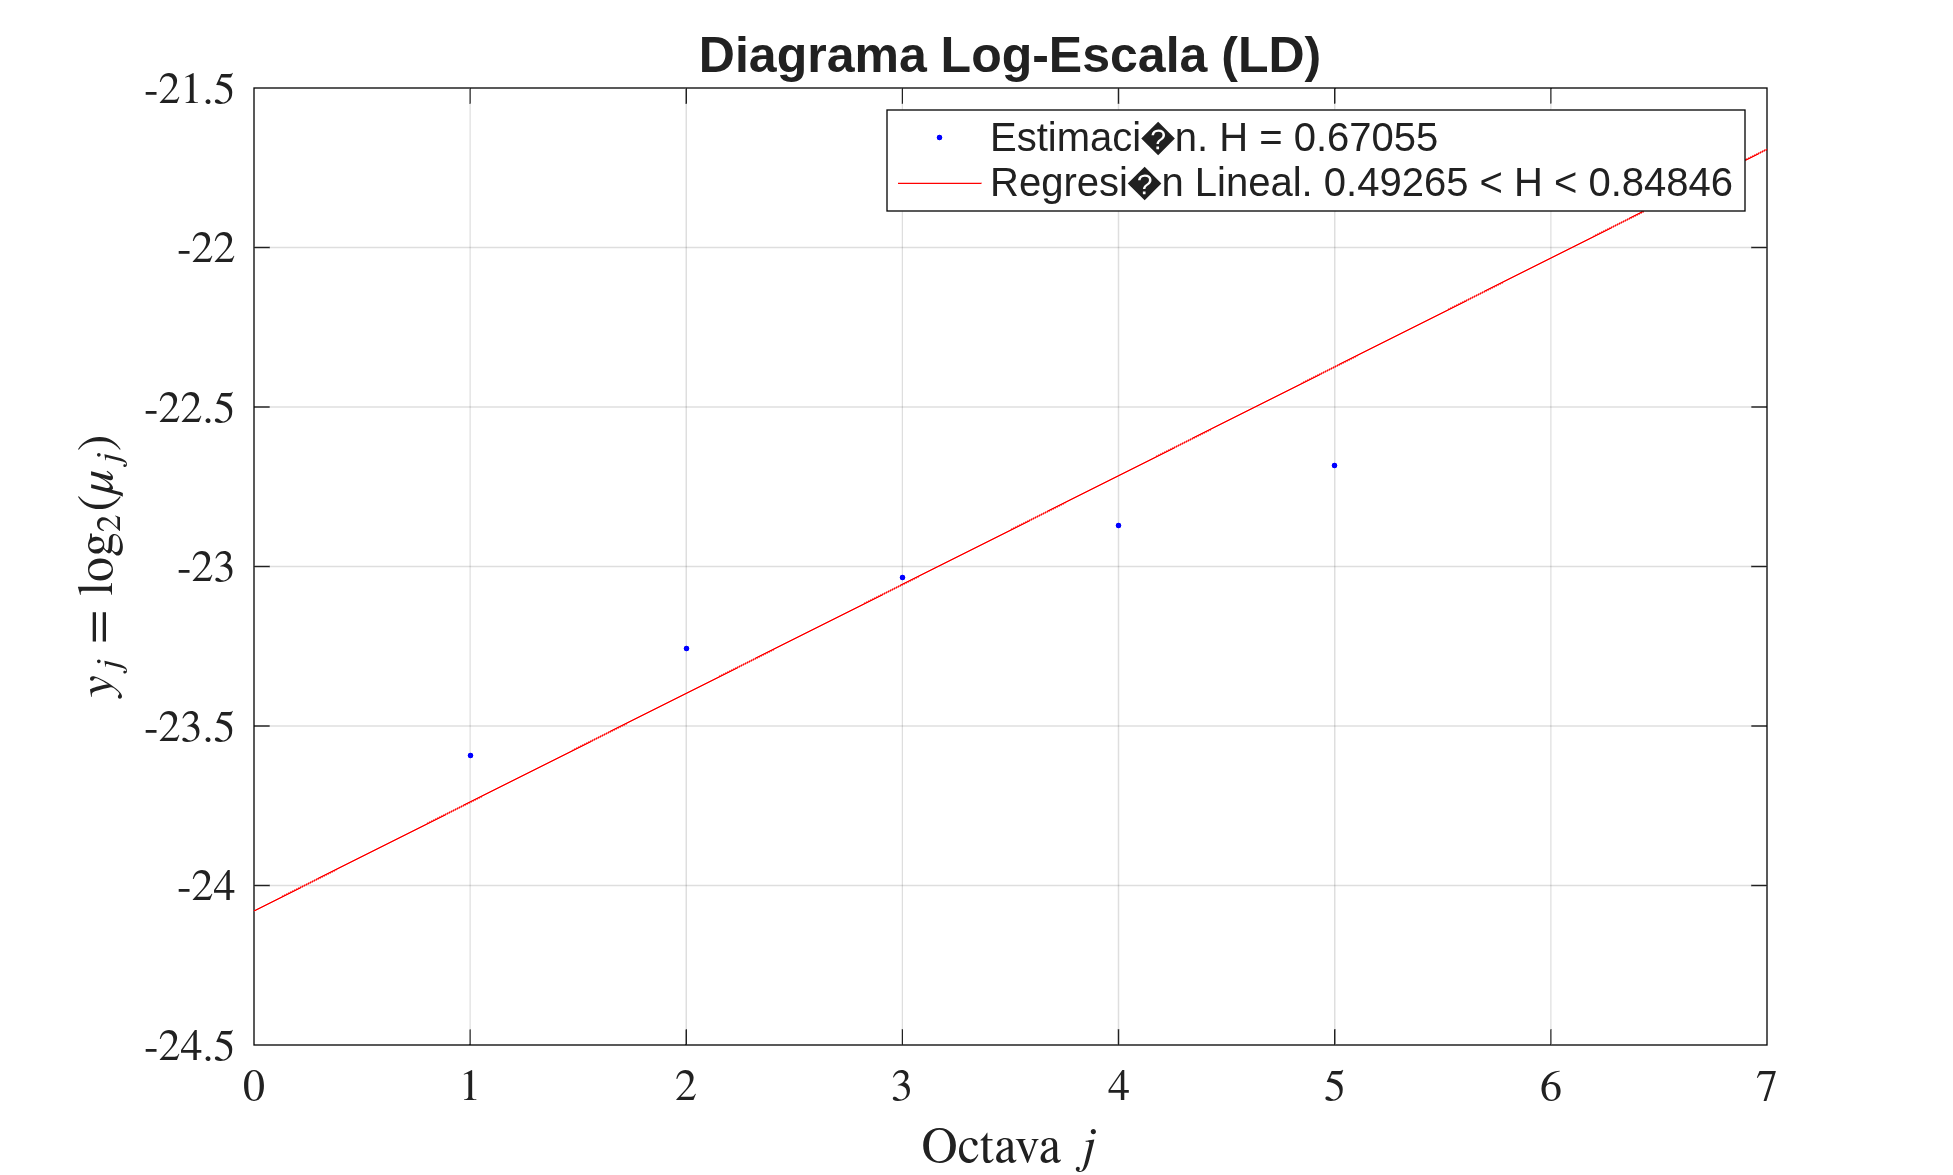
\includegraphics[width=\textwidth]{actividades/actividad6/imgs/btc_diagrama_ld.png}
        \caption{Anexo A.2: Diagrama LD de volatilidad BTC/USDT.}
    \end{minipage}
\end{figure}

\begin{figure}[H]
    \centering
    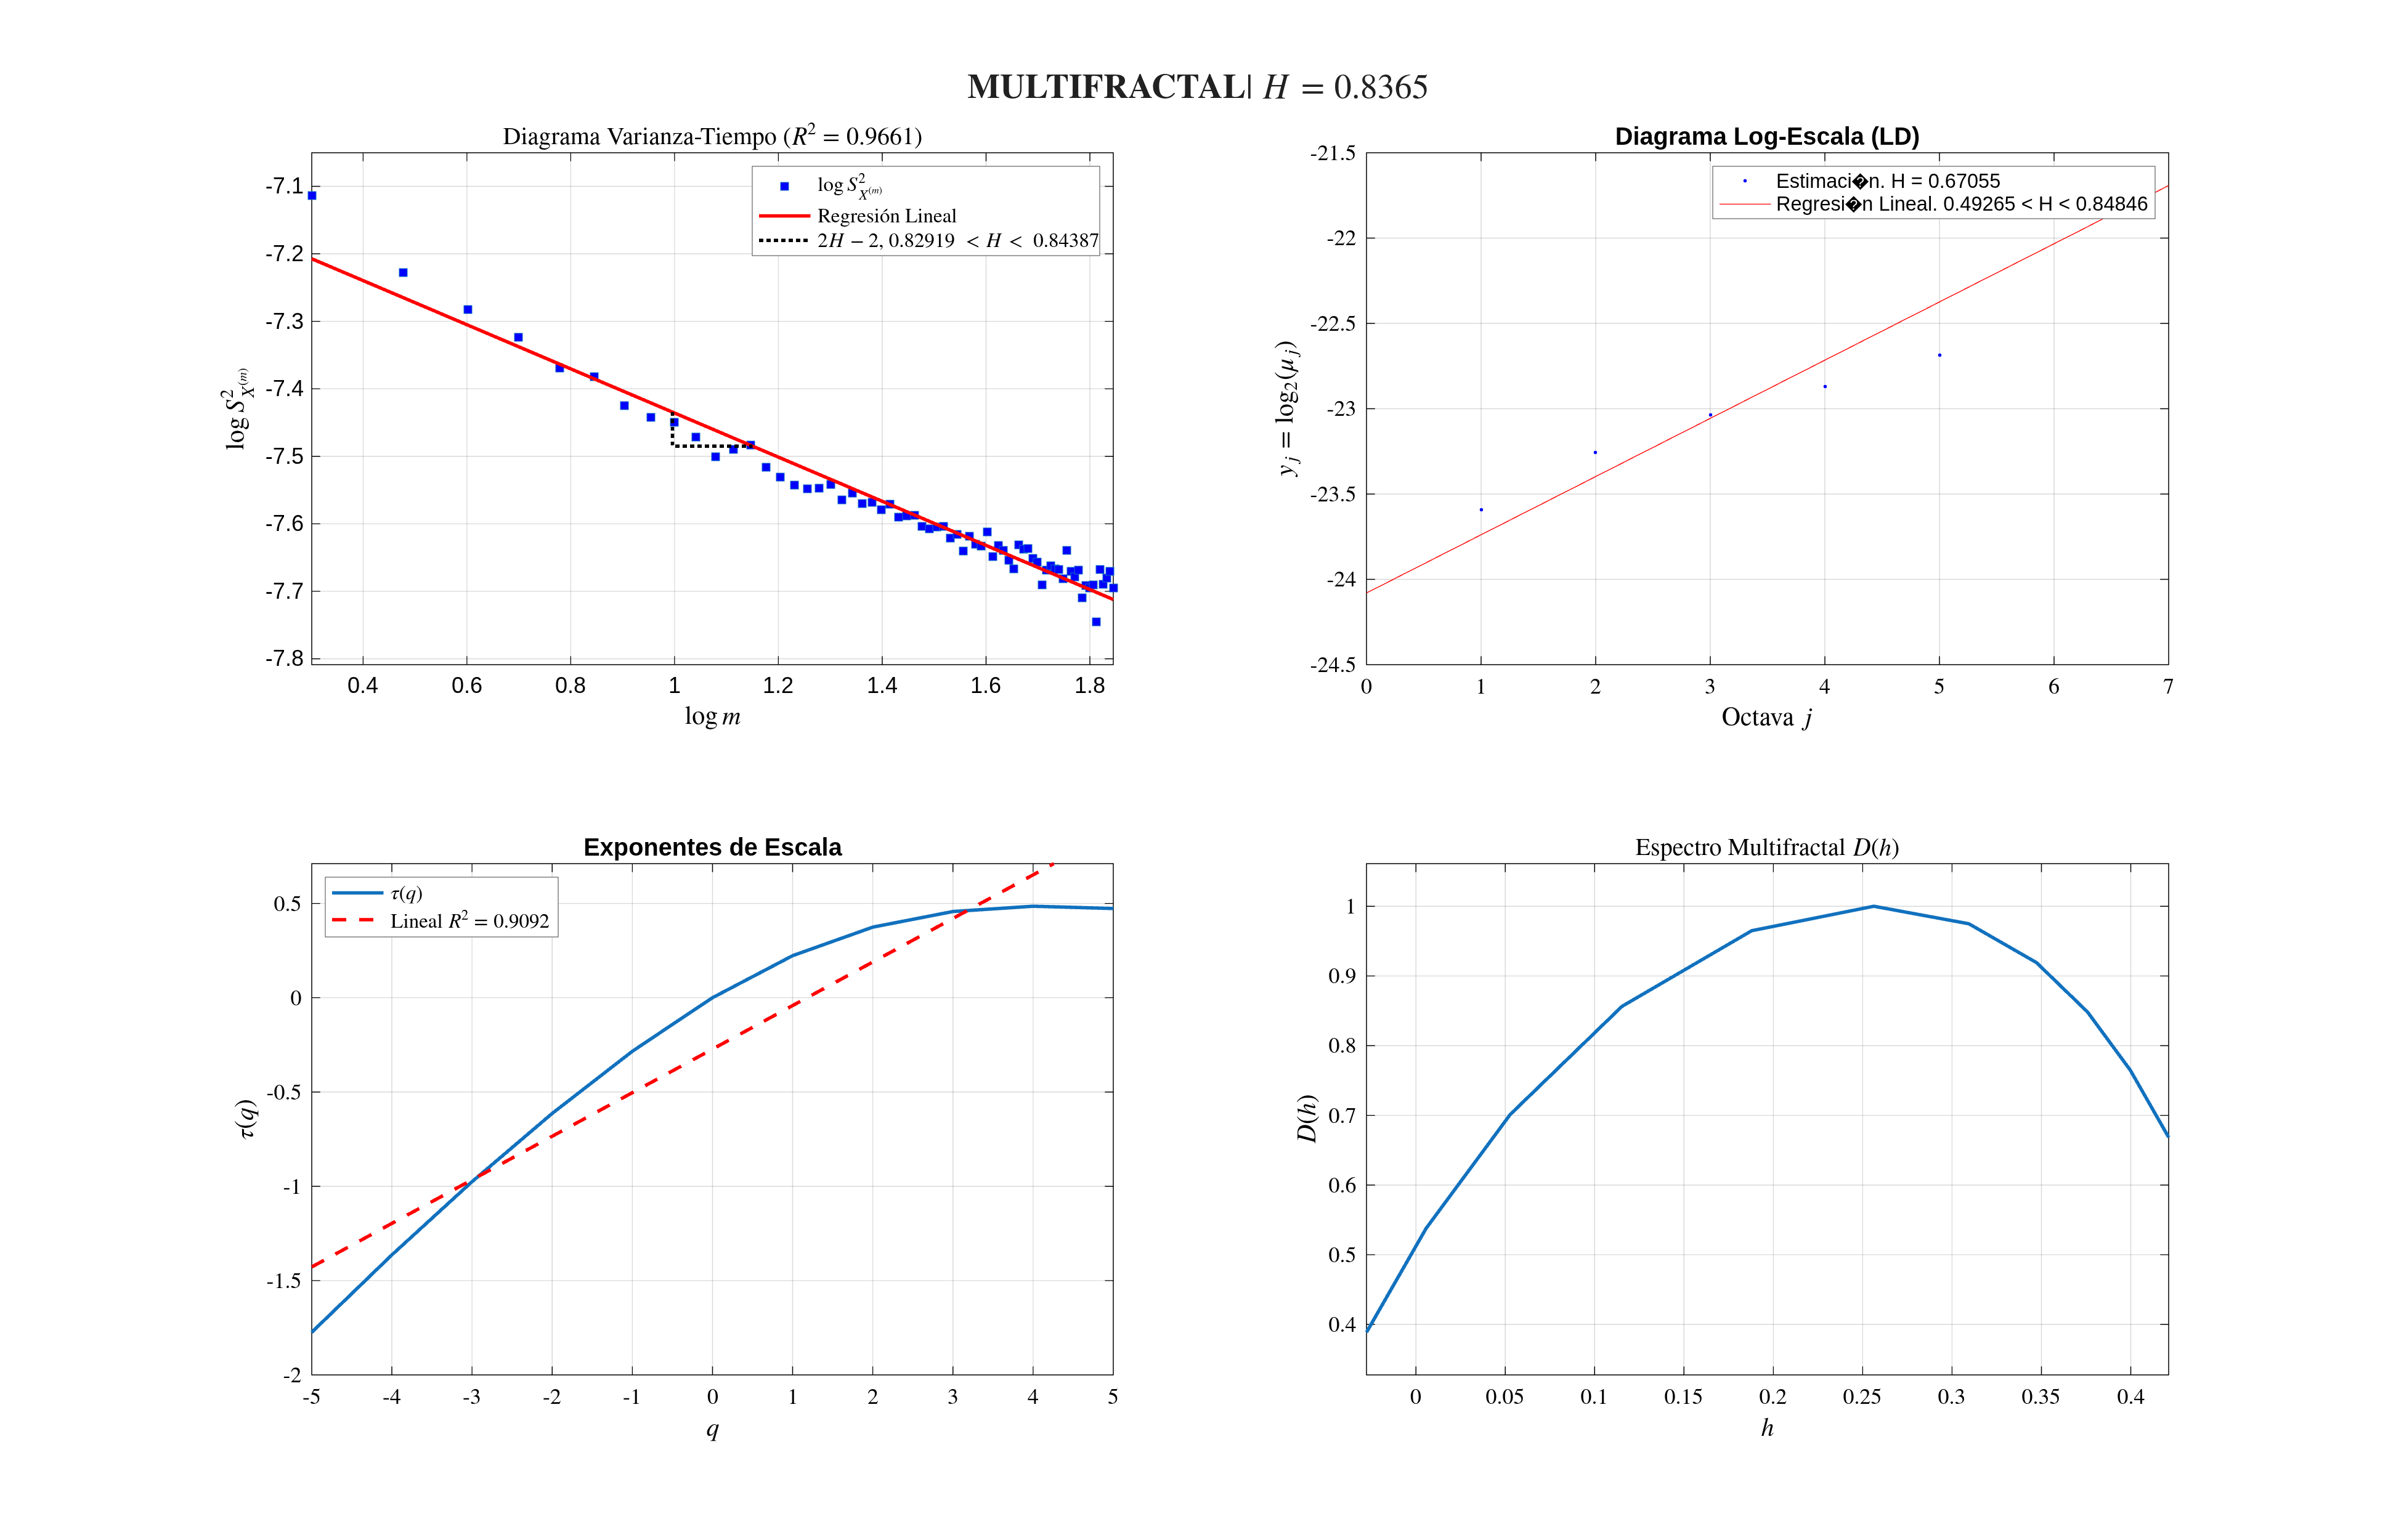
\includegraphics[width=0.85\textwidth]{actividades/actividad6/imgs/btc_clasificacion_fractal.png}
    \caption{Anexo A.2: Clasificaci\'{o}n multifractal de volatilidad BTC/USDT.}
\end{figure}

% ------------------------------------------------------------
\subsection*{A.3 Resumen comparativo de experimentos complementarios}
% ------------------------------------------------------------

\begin{table}[H]
\centering
\caption{Resumen de experimentos complementarios.}
\begin{tabular}{lcccccc}
\toprule
\textbf{Dataset} & $n$ & $\hat{H}_{\text{VT}}$ & $\hat{H}_{\text{LD}}$ & $R^2_{\text{VT}}$ & $R^2_{\tau}$ & \textbf{Clasif.} \\
\midrule
FRED DGS10 (diff)  & 16\,801 & 0{,}5185 & 0{,}5826 & 0{,}9858 & 0{,}8925 & Multifractal \\
BTC/USDT (vol)     & 4\,999  & 0{,}8365 & 0{,}6706 & 0{,}9661 & 0{,}9092 & Multifractal \\
\bottomrule
\end{tabular}
\end{table}

Los resultados de los anexos A.1 y A.2 complementan el an\'{a}lisis
principal de la Actividad~6 (S\&P~500) al confirmar que:
\begin{enumerate}[leftmargin=2em, nosep]
    \item La LRD en volatilidad financiera es robusta ante cambios de
          activo (\'{i}ndices tradicionales vs.~criptoactivos).
    \item La LRD en diferencias de tasas soberanas es m\'{a}s modesta,
          sugiriendo que la regulaci\'{o}n centralizada diluye la memoria
          persistente en las fluctuaciones de corto plazo.
    \item La multifractalidad es la norma en sistemas financieros reales;
          el resultado monofractal del S\&P~500 (Actividad~6) puede
          reflejar la dominancia de un \'{u}nico mecanismo de escalamiento
          en horizontes diarios de 24 a\~{n}os.
\end{enumerate}
